% Round 3 agent architecture (usagi), one page.
% Build:  ~/miniconda3/envs/latex/bin/tectonic architecture.tex   -> architecture.pdf
%
% SKELETON: boxes, arrows and labels are code names and facts taken from the files in this folder
% (agent.json, strategist.py, restock.py, seller_r3.py, market_buyer.py, review.py, market_tool.py) and the kit
% (market_kit.py, starter_round3). The explanation of the structure and of how it differs from the kit default
% was filled in on 11-23 (orange = where the model is called). Korean text works (XeTeX + Noto Sans CJK KR).
\documentclass[tikz,border=10pt]{standalone}
\usepackage{fontspec}
\setmainfont{Noto Sans CJK KR}
\setmonofont{Noto Sans Mono CJK KR}
\usetikzlibrary{positioning,fit,arrows.meta,backgrounds,calc}

\tikzset{
  box/.style={draw, rounded corners=2pt, align=center, inner sep=4pt, font=\small, minimum height=11mm},
  model/.style={box, fill=orange!15, draw=orange!70!black, thick},
  code/.style={box, fill=blue!7, draw=blue!60!black},
  file/.style={draw, align=left, inner sep=3pt, font=\scriptsize\ttfamily, fill=gray!8},
  ext/.style={box, fill=green!8, draw=green!45!black},
  group/.style={draw, dashed, rounded corners=6pt, inner sep=8pt, inner ysep=10pt},
  glabel/.style={font=\small\bfseries, anchor=south west, inner sep=2pt},
  flow/.style={-{Stealth[length=2.2mm]}, thick},
  ctrl/.style={-{Stealth[length=2.2mm]}, thick, densely dashed, orange!70!black},
  lbl/.style={font=\scriptsize, fill=white, inner sep=1pt},
}

\begin{document}
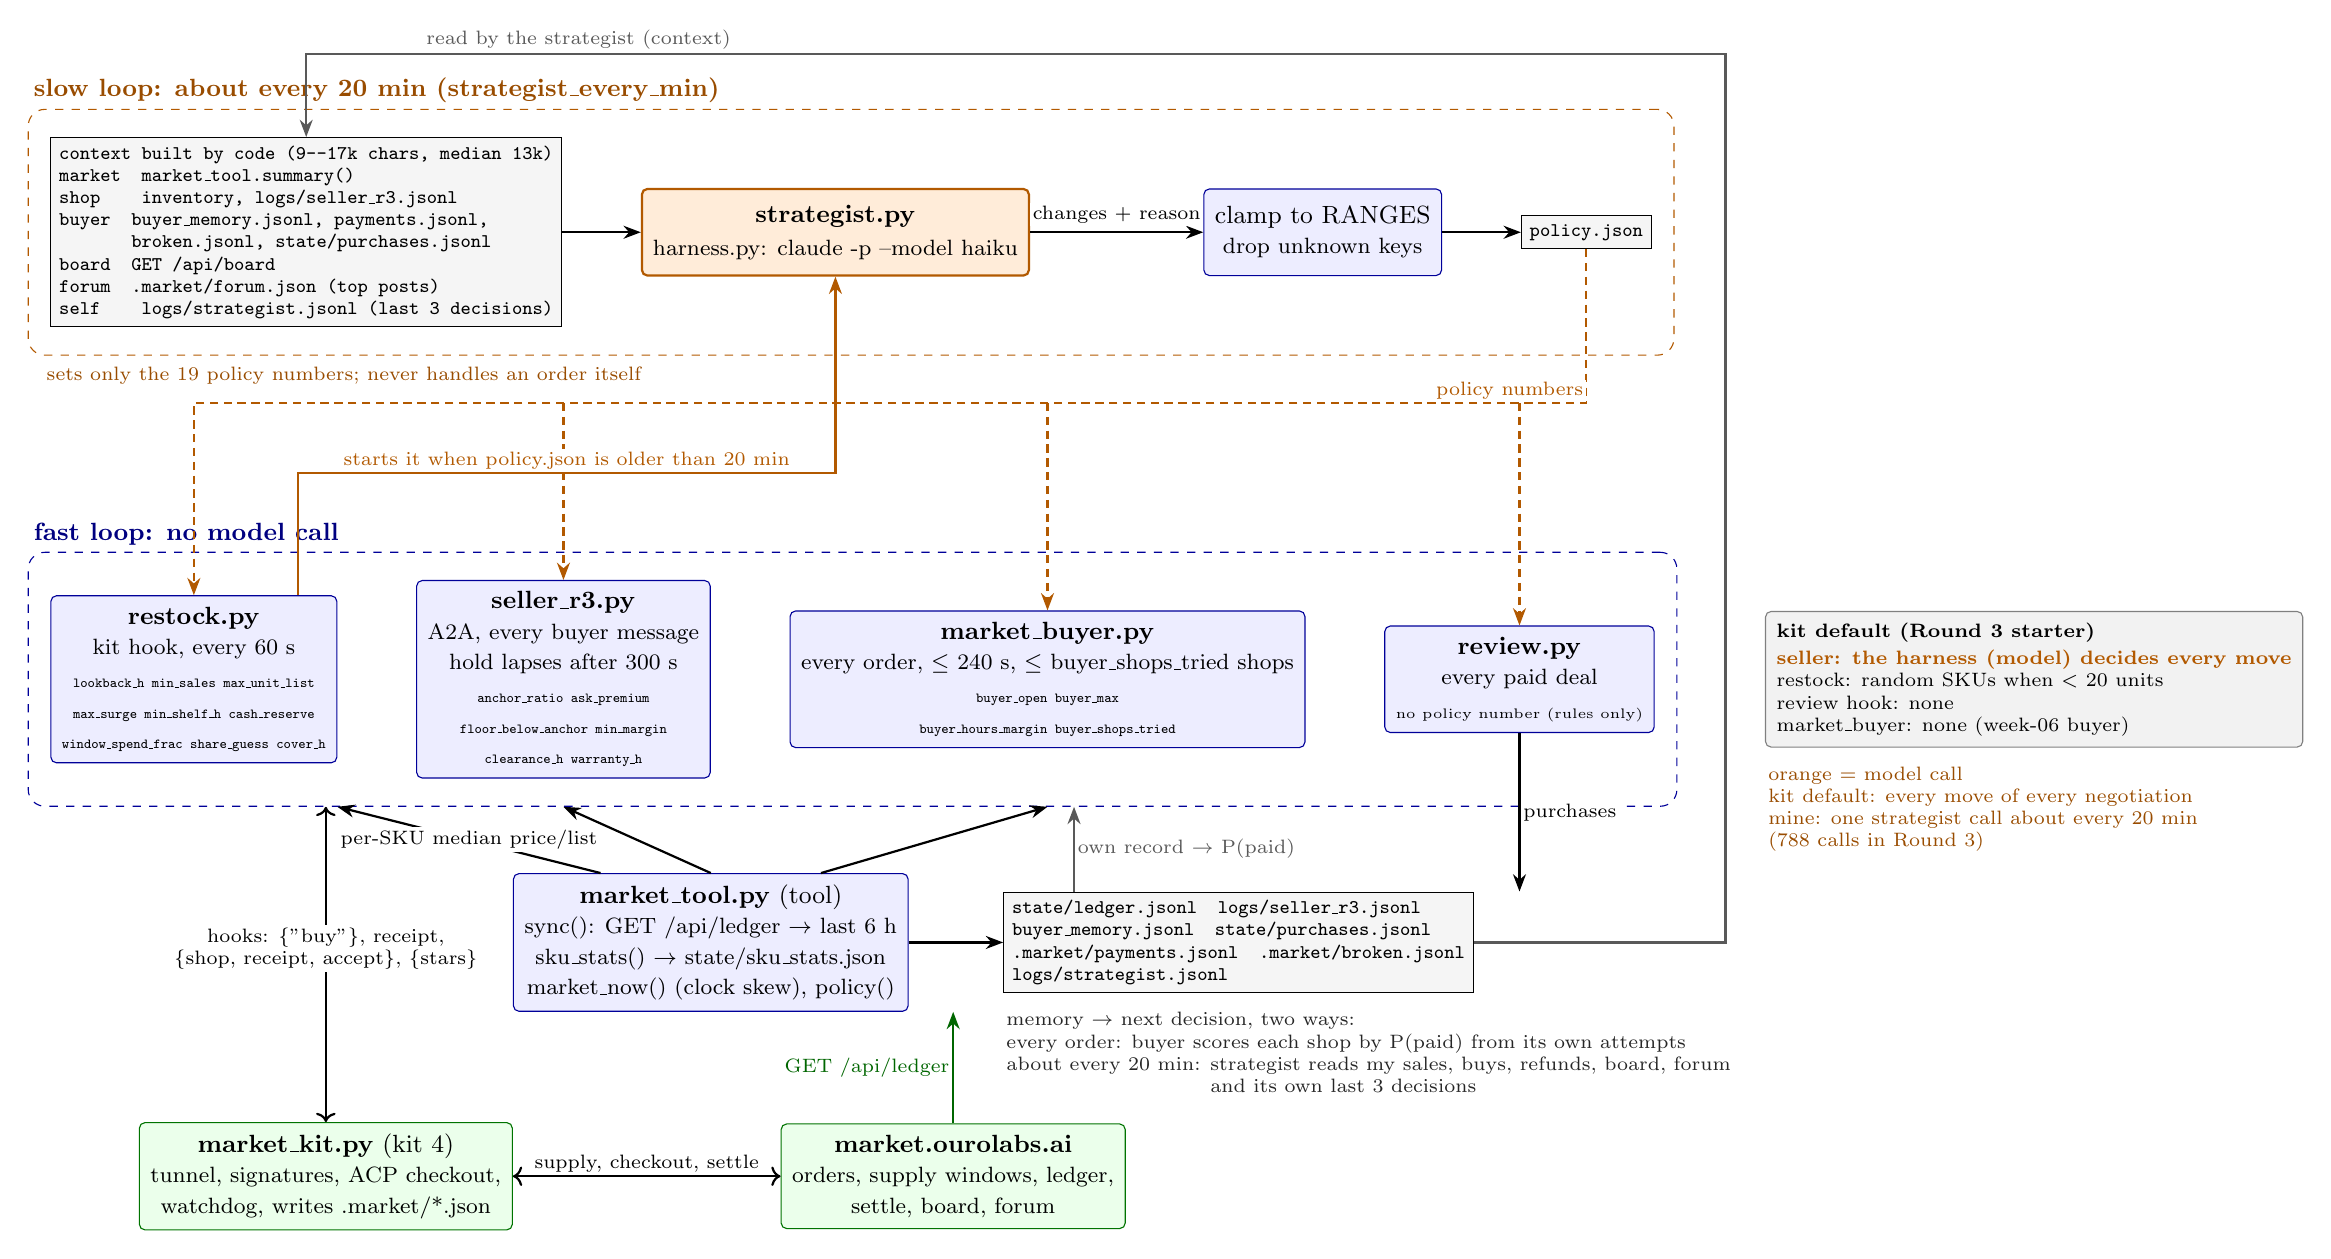
\begin{tikzpicture}[node distance=8mm and 10mm]

% ---------------- slow loop: the one model call ----------------
\node[file] (ctx) {context built by code (9--17k chars, median 13k)\\
  market\quad market\_tool.summary()\\
  shop\quad\ \ inventory, logs/seller\_r3.jsonl\\
  buyer\quad buyer\_memory.jsonl, payments.jsonl,\\
  \phantom{buyer}\quad broken.jsonl, state/purchases.jsonl\\
  board\quad GET /api/board\\
  forum\quad .market/forum.json (top posts)\\
  self\quad\ \ logs/strategist.jsonl (last 3 decisions)};
\node[model, right=of ctx] (strat) {\textbf{strategist.py}\\[1pt]\footnotesize harness.py: claude -p --model haiku};
\node[code, right=22mm of strat] (clamp) {clamp to RANGES\\\footnotesize drop unknown keys};
\node[file, right=of clamp] (policy) {policy.json};
\draw[flow] (ctx) -- (strat);
\draw[flow] (strat) -- node[lbl, above=2pt] {changes + reason} (clamp);
\draw[flow] (clamp) -- (policy);
\begin{scope}[on background layer]
  \node[group, draw=orange!70!black, fit=(ctx)(strat)(clamp)(policy)] (slow) {};
\end{scope}
\node[glabel, text=orange!60!black] at (slow.north west) {slow loop: about every 20 min (strategist\_every\_min)};
\node[font=\scriptsize, text=orange!60!black, anchor=north west, inner sep=1pt] at ($(slow.south west)+(2mm,-1mm)$) {sets only the 19 policy numbers; never handles an order itself};

% ---------------- fast loop: code only ----------------
\node[code, below=34mm of ctx.south west, anchor=north west] (restock) {\textbf{restock.py}\\\footnotesize kit hook, every 60 s\\[1pt]\tiny\ttfamily lookback\_h min\_sales max\_unit\_list\\\tiny\ttfamily max\_surge min\_shelf\_h cash\_reserve\\\tiny\ttfamily window\_spend\_frac share\_guess cover\_h};
\node[code, right=of restock] (seller) {\textbf{seller\_r3.py}\\\footnotesize A2A, every buyer message\\\footnotesize hold lapses after 300 s\\[1pt]\tiny\ttfamily anchor\_ratio ask\_premium\\\tiny\ttfamily floor\_below\_anchor min\_margin\\\tiny\ttfamily clearance\_h warranty\_h};
\node[code, right=of seller] (buyer) {\textbf{market\_buyer.py}\\\footnotesize every order, $\le$ 240 s, $\le$ buyer\_shops\_tried shops\\[1pt]\tiny\ttfamily buyer\_open buyer\_max\\\tiny\ttfamily buyer\_hours\_margin buyer\_shops\_tried};
\node[code, right=of buyer] (review) {\textbf{review.py}\\\footnotesize every paid deal\\[1pt]\tiny no policy number (rules only)};
\begin{scope}[on background layer]
  \node[group, draw=blue!60!black, fit=(restock)(seller)(buyer)(review)] (fast) {};
\end{scope}
\node[glabel, text=blue!50!black] at (fast.north west) {fast loop: no model call};
% each executor box lists the policy numbers it reads (9 + 6 + 4 = 19, checked against the code)

\coordinate (busY) at ($(slow.south)+(0,-6mm)$);
\coordinate (trigY) at ($(fast.north)+(0,10mm)$);
\draw[ctrl] (policy.south) -- (policy.south |- busY) -| (restock.north);
\foreach \n in {seller, buyer, review} \draw[ctrl] (\n.north |- busY) -- (\n.north);
\node[lbl, text=orange!70!black, anchor=south east] at (policy.south |- busY) {policy numbers};
\coordinate (trigS) at ($(restock.north east)+(-5mm,0)$);
\draw[flow, orange!70!black] (trigS) -- (trigS |- trigY)
  -| node[lbl, pos=0.25, above] {starts it when policy.json is older than 20 min} (strat.south);

% ---------------- kit default, for comparison ----------------
\node[box, fill=gray!10, draw=gray, align=left, font=\scriptsize, right=14mm of review] (base) {\textbf{kit default (Round 3 starter)}\\[2pt]
  \textcolor{orange!70!black}{\textbf{seller: the harness (model) decides every move}}\\
  restock: random SKUs when $<$ 20 units\\
  review hook: none\\
  market\_buyer: none (week-06 buyer)};
\node[font=\scriptsize, text=orange!60!black, align=left, anchor=north west, inner sep=1pt] at ($(base.south west)+(0,-2mm)$) {orange = model call\\kit default: every move of every negotiation\\mine: one strategist call about every 20 min\\(788 calls in Round 3)};

% ---------------- tool and memory ----------------
\node[code, below=12mm of seller.south east, anchor=north] (tool) {\textbf{market\_tool.py} (tool)\\\footnotesize sync(): GET /api/ledger $\rightarrow$ last 6 h\\\footnotesize sku\_stats() $\rightarrow$ state/sku\_stats.json\\\footnotesize market\_now() (clock skew), policy()};
\node[file, right=12mm of tool] (mem) {state/ledger.jsonl\quad logs/seller\_r3.jsonl\\
  buyer\_memory.jsonl\quad state/purchases.jsonl\\
  .market/payments.jsonl\quad .market/broken.jsonl\\
  logs/strategist.jsonl};
\draw[flow] (tool) -- (mem);
\draw[flow] (tool.north) ++(-14mm,0) -- node[lbl] {per-SKU median price/list} (restock.south east |- fast.south);
\draw[flow] (tool.north) -- (seller.south |- fast.south);
\draw[flow] (tool.north) ++(14mm,0) -- (buyer.south |- fast.south);
\draw[flow] (review.south) -- node[lbl, right] {purchases} (review.south |- mem.north);
\coordinate (memB) at ($(mem.north west)+(9mm,0)$);
\draw[flow, gray!70!black] (memB) -- node[lbl, right] {own record $\rightarrow$ P(paid)} (memB |- fast.south);
\draw[flow, gray!70!black] (mem.east) -| ($(base.west)+(-5mm,0)$) |- ($(slow.north)+(0,7mm)$) -| node[lbl, pos=0.25, above] {read by the strategist (context)} (ctx.north);
\node[font=\scriptsize, text=gray!30!black, align=left, anchor=north west, inner sep=1pt] at ($(mem.south west)+(0,-2mm)$) {memory $\rightarrow$ next decision, two ways:\\every order: buyer scores each shop by P(paid) from its own attempts\\about every 20 min: strategist reads my sales, buys, refunds, board, forum\\\phantom{about every 20 min: }and its own last 3 decisions};

% ---------------- kit and market ----------------
\node[ext, below=14mm of tool.south west, anchor=north east] (kit) {\textbf{market\_kit.py} (kit 4)\\\footnotesize tunnel, signatures, ACP checkout,\\\footnotesize watchdog, writes .market/*.json};
\node[ext, right=34mm of kit] (market) {\textbf{market.ourolabs.ai}\\\footnotesize orders, supply windows, ledger,\\\footnotesize settle, board, forum};
\draw[flow, <->] (kit) -- node[lbl, above] {supply, checkout, settle} (market);
\draw[flow, <->] (kit.north) -- node[lbl, pos=0.55, align=center] {hooks: \{"buy"\}, receipt,\\\{shop, receipt, accept\}, \{stars\}} (fast.south -| kit.north);
\draw[flow, green!40!black] (market.north) -- node[lbl, left] {GET /api/ledger} (market.north |- tool.south);

\end{tikzpicture}
\end{document}
